\begin{figure*}
    \centering
    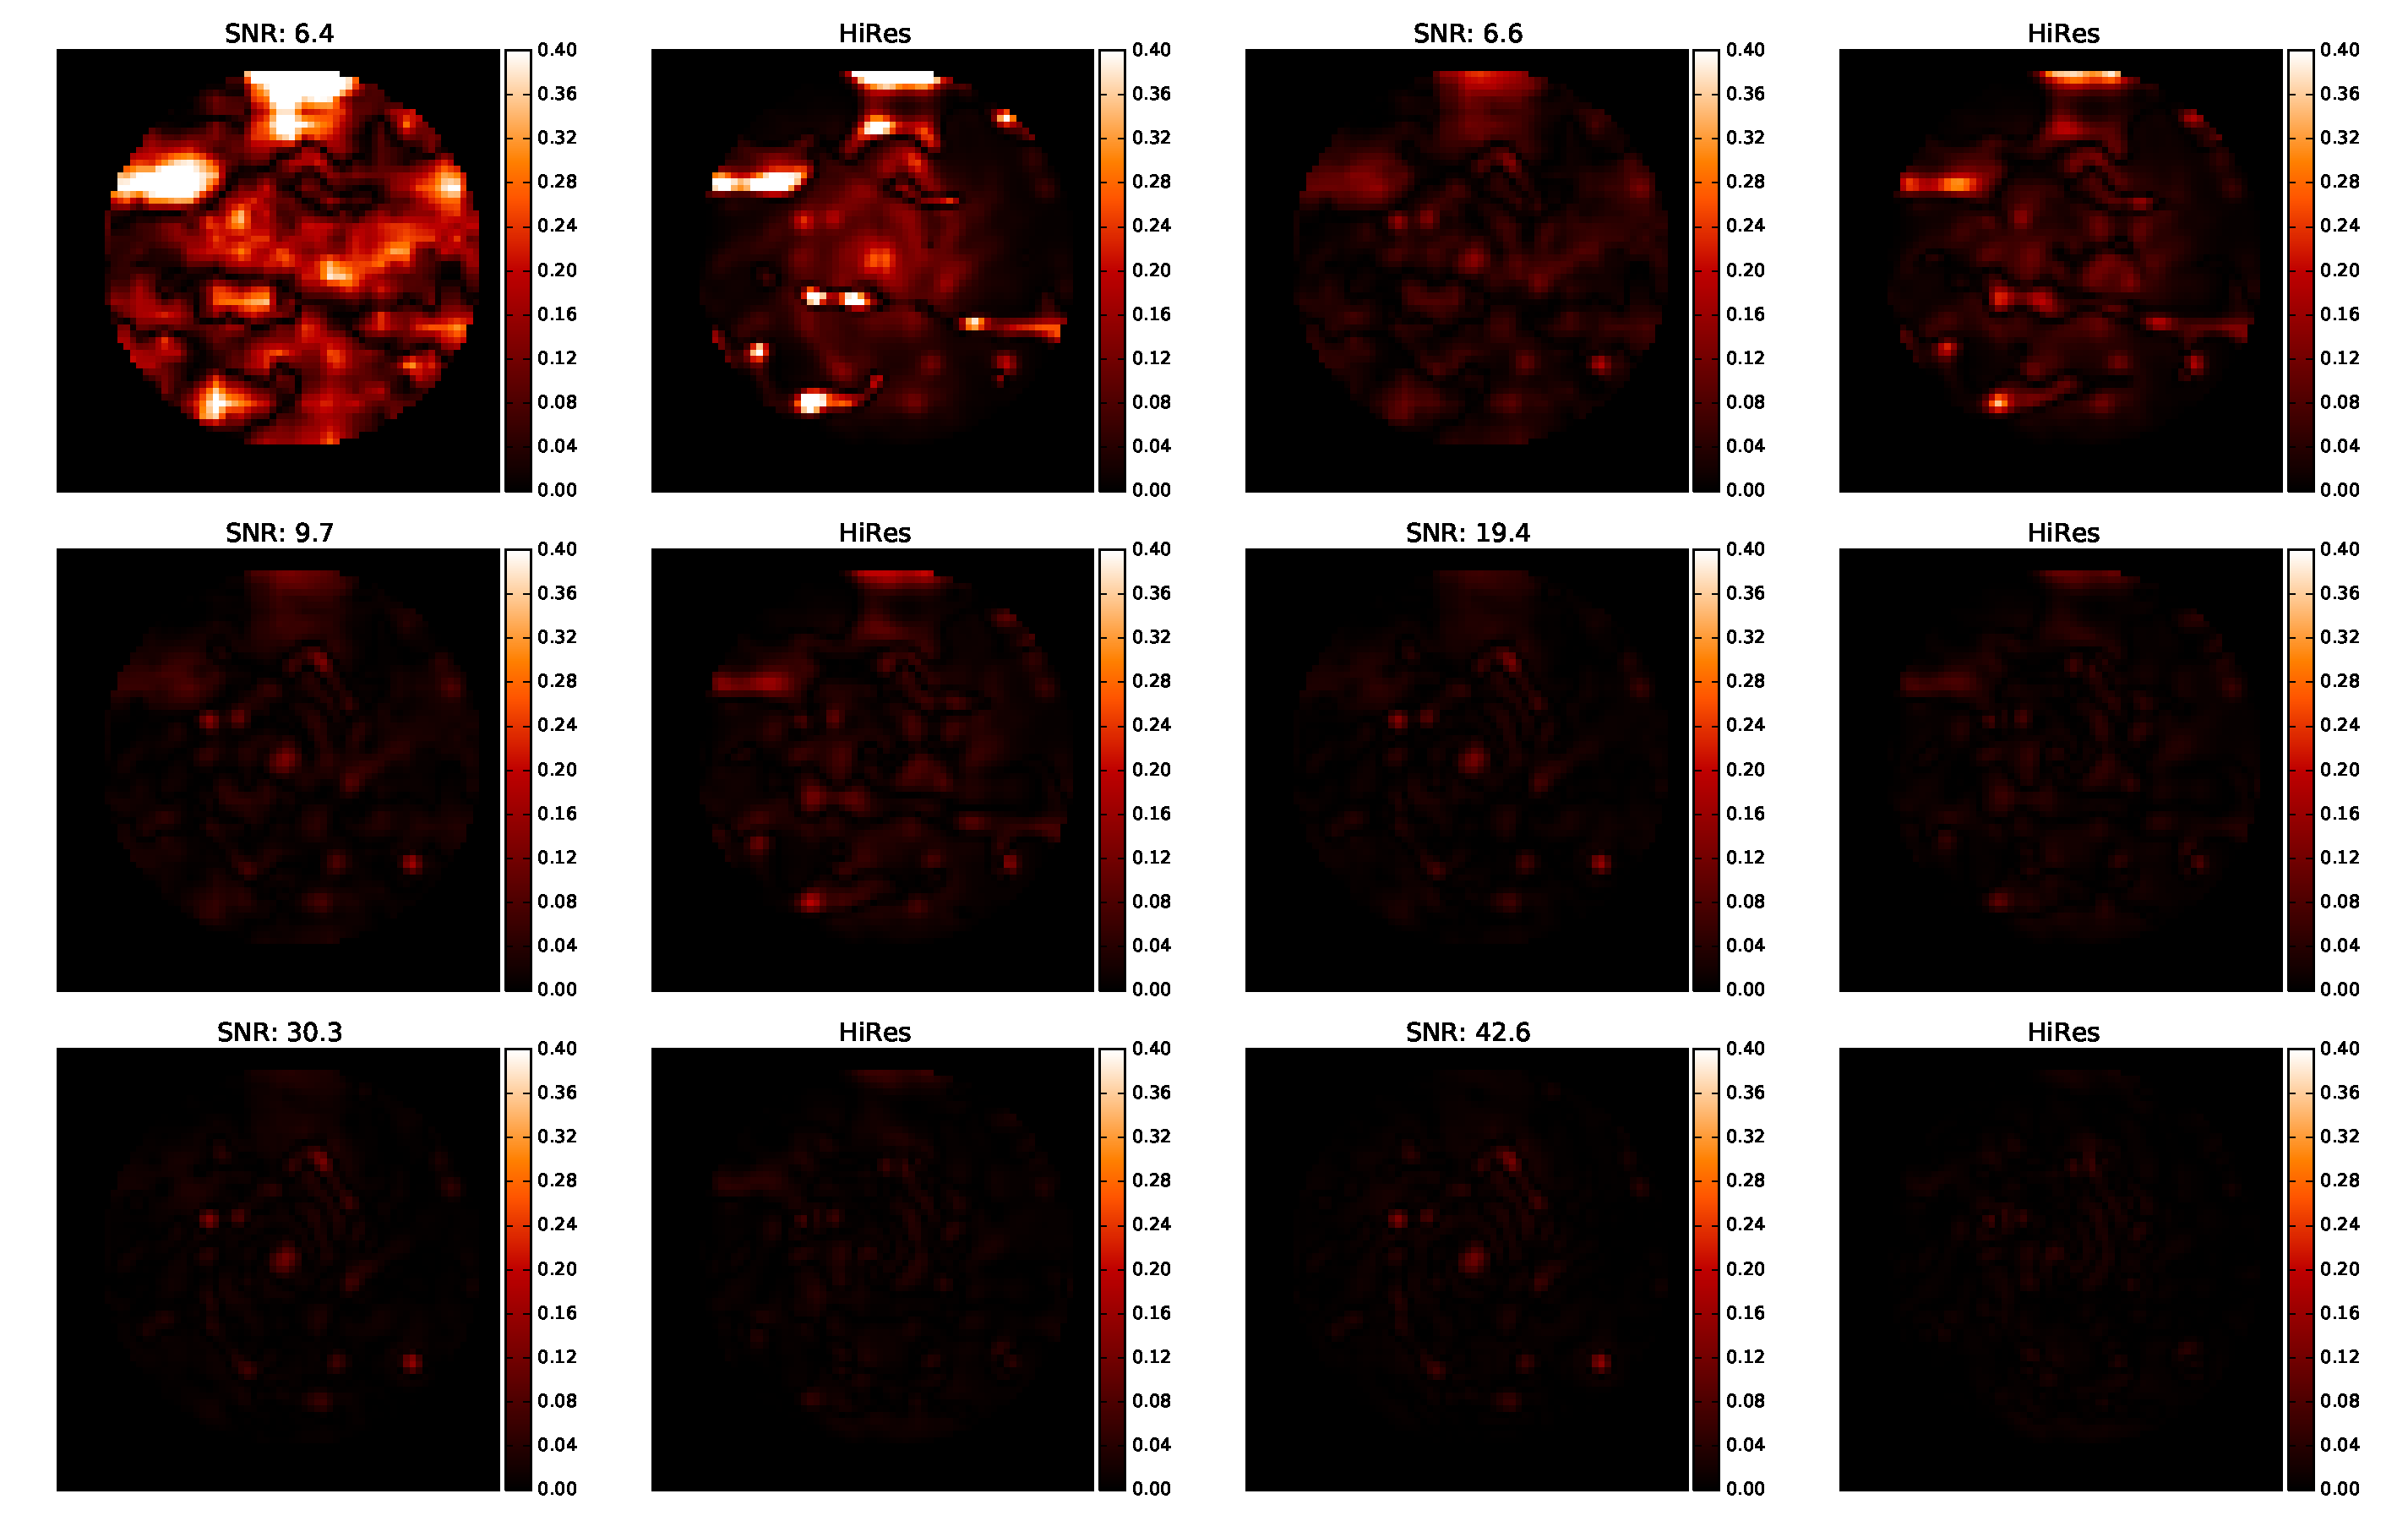
\includegraphics[width=0.85\linewidth]{figures/diff_maps.pdf}
    \caption[Difference Maps]{Difference Maps at various SNR, showing both simulated and HiRes image differences. All are shown with the same color scale, clearly demonstrating how the pixel difference decreases as SNR increases. Each pair of images is the pixel difference for the simulation and the HiRes output on that observation. All values are in Jy/beam}
    \label{diffmaps}
\end{figure*}

To clarify the terminology in this section, 'simulation' refers to the observation created from Spitzer data convolved with the SPIRE beam, 'HiRes' is the output of the HiRes routine on the simulation data, and 'truth' is the observation created from the Spitzer data convolved with the half-size SPIRE beam. When talking about any difference image, these are always taken as the data from the truth image, with either the simulation or HiRes image maps subtracted.

As we have generated a theoretical truth image it is possible to simply measure pixel differences between this truth and the output of the HiRes routines on the simulation data. By looking at the RMS (root-mean-square) pixel difference for a particular sample  it is possible to arrive at a simple number that can be used as a basis of comparison. Then, by examining the RMS pixel difference as a function of the peak signal to noise, a condition can be arrived at for when it is suitable to use HiRes on an observation.

It is not simply enough just to compare the maps as created, as in that case the RMS pixel difference would just be a function of the noise regime used in the simulation. Instead, the images need to be flux normalized and have an aperture placed over the region of interest. In the case of the M74 simulation an aperture is placed over the central galaxy, so that we are not simply comparing the noise in the background window. The total flux is then normalized between both images, and the RMS pixel difference is measured.

So the first step is to put an aperture over the image. This is done by (in the case of my data) generating a mask image that has the same dimensions as the data images. Each location in the mask is then assigned either a 0 or 1 value depending on location. Any pixel inside a radius of 30 pixels around the centre of the galaxy is assigned 1, and every pixel outside this region is assigned a value of 0. This image can then be multiplied to any other image to mask out regions outside of this zone of interest. The sum of the mask also conveniently gives the total number of pixels inside the zone of interest and can be used for instance in the calculation of averages.

Secondly the flux between the masked images needs to be normalized. In the case of two images, subscripted as 1 and 2, the data can be normalized such that they both contain the same total flux as shown in equation \ref{imnorm}.

\begin{equation}
     I_{1,x,y} = I_{1,x,y} \times \frac{\sum\limits_{x,y}{I_{2,x,y}}}{\sum\limits_{x,y}{I_{1,x,y}}}
     \label{imnorm}
\end{equation}

Once they are normalized, the simulation and original images can be subtracted from the truth image (figure \ref{diffmaps}, and the root mean square of the resulting difference maps can be calculated. Performing this analysis for the range of simulation images produced gives the result shown in figure \ref{diffresults}. As the same processing has been performed for a variety of regions in the background map, the error simply shows the standard deviation of the RMS value for each SNR sample. This also shows how the HiRes routine does reduce the flux in the background regions as the error is much less sensitive to the differences in background map itself.

\begin{figure}[H]
    \centering
    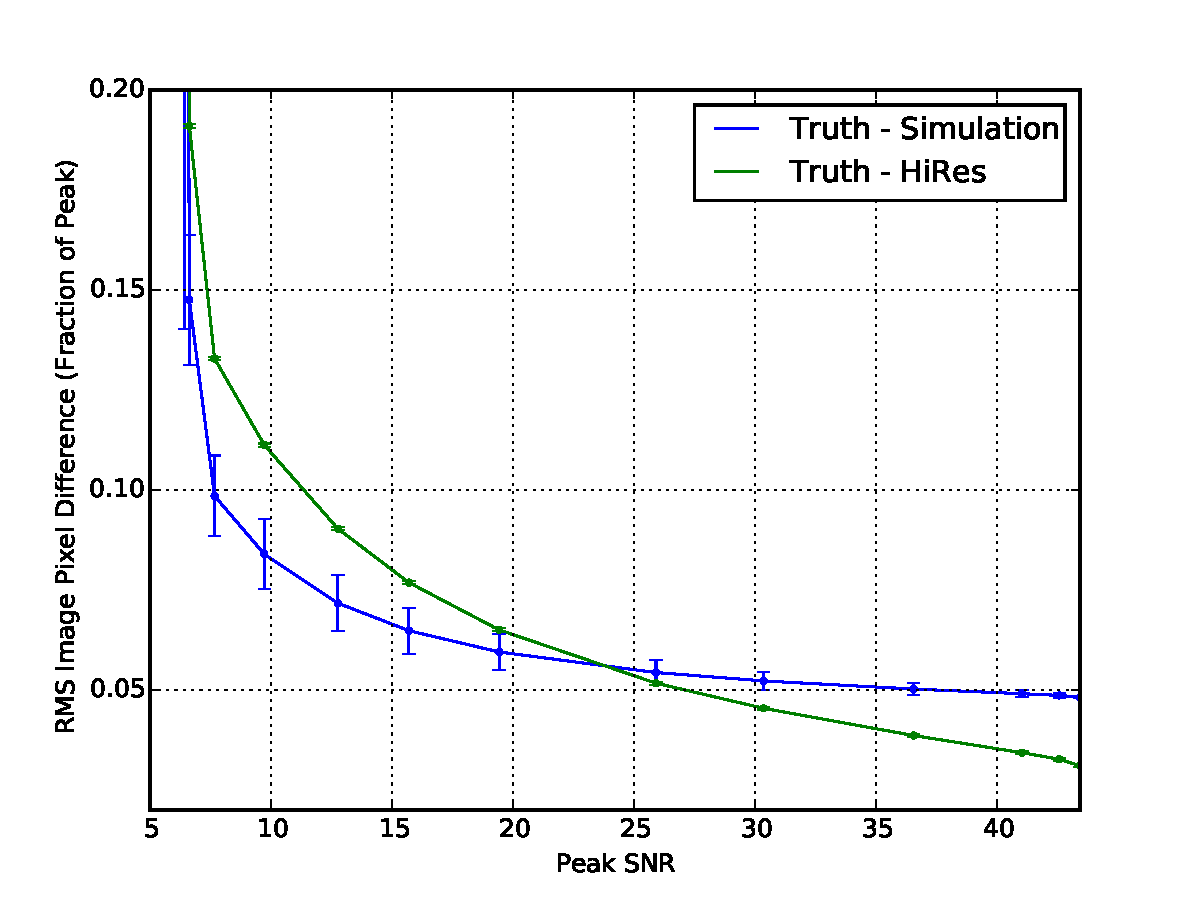
\includegraphics[width=\linewidth]{figures/differences.pdf}
    \caption[RMS Pixel differences as a function of peak SNR]{RMS Pixel differences as a function of peak SNR for the difference maps of both the simulated observations against the truth image, and the HiRes output of the simulations against the truth image. Clearly showing that for low SNR HiRes actually decreases the fidelity of the observation, but above an SNR of 30 a noticeable improvement occurs, rising rapidly as SNR further increases.}
    \label{diffresults}
\end{figure}

As shown in figure \ref{diffresults}, at low peak SNR (\textless 25) HiRes actually reduces the quality of the produced maps, as the RMS pixel difference is actually higher than when the difference is taken just for the simulation image. It is not until rising above a peak SNR of approximately 30 that the maps produced actually become better than the simulated observations themselves, and this improvement continues rapidly, rising to about a 40\% reduction in the RMS pixel difference betweek the simulated observation and the HiRes processed observation at a SNR above 40.
